\documentclass{beamer}

\usepackage{amsmath,amssymb}
\usepackage{tikz}
\usepackage{graphicx}
\usepackage{multicol}
\usepackage[per-mode=fraction]{siunitx}

\usetheme{Boadilla}
\usecolortheme{orchid}

\usetikzlibrary{calc,math}
\usetikzlibrary{positioning}
\usetikzlibrary{decorations.markings}
\usetikzlibrary{angles,quotes}

\tikzset{>=stealth,
  coord/.style = {circle,fill=black,draw=black,minimum size=0.1cm,inner sep=0pt},
  tangent/.style={
    decoration={
      markings,
      mark = at position #1
           with{
             \coordinate (tangent point-\pgfkeysvalueof{/pgf/decoration/mark info/sequence number})
                                     at (0pt,0pt);
        \coordinate (tangent unit vector-\pgfkeysvalueof{/pgf/decoration/mark info/sequence number}) at (1,0pt);
        \coordinate (tangent orthogonal unit vector-\pgfkeysvalueof{/pgf/decoration/mark info/sequence number}) at (0pt,1);
      }
    },
    postaction=decorate
  },
  use tangent/.style={
    shift=(tangent point-#1),
    x=(tangent unit vector-#1),
    y=(tangent orthogonal unit vector-#1)
  },
  use tangent/.default=1
}

\title{PHYS2350: Motion in 2D}
\author{Dr. Wolf}
\date{Fall 2024}

\begin{document}

\begin{frame}
  \titlepage
\end{frame}

\begin{frame}
  {Group discussion: Direction of velocity vector}

  Suppose you are traveling along the indicated path from point A to point B at a constant
  speed of \SI{3}{\meter\per\second}. Which direction is the velocity at point C? How do you
  know?

  \begin{center}
    \begin{tikzpicture}
      \coordinate (A) at (0,5);
      \coordinate (B) at (5,0);
      \coordinate (C) at (6,3);
      \fill (A) circle (0.05) node [above left]{A};
      \fill (B) circle (0.05) node [below right]{B};
      \fill (C) circle (0.05) node [left]{C};

      \draw (A) .. controls +(10:3) and +(80:2) .. (C) .. controls +(-100:2) and +(+100:3)
      .. (B);

      \onslide<2->{
        \draw[->,blue,thick] (C) -- +(-100:2) node[midway,right]{$\vec{v}_C$};
      }
      \onslide<3->{
        \node[blue] at (-1,2) {Not sure why\ldots but that \textit{is} correct};
      }
      \onslide<4->{
        \node[red] at (-1,0.5) {And that's what page 1 is all about.};
      }
    \end{tikzpicture}
  \end{center}
\end{frame}

\begin{frame}
  {Direction of the instantaneous velocity is tangent to the curve}
  \only<1-2>{
    \textbf{Step \#1} Draw $\vec{r}_A$ and $\vec{r}_B$, the position vectors for the object when
    it is at point A and B \textit{relative to the origin} O.
  }
  \only<3-7>{
    \textbf{Step \#2} Draw the vector that represents the \textit{displacement} of the object
    from A to B.
    \uncover<4-7>{
      $$\Delta\vec{r}_{AB} = \vec{r}_B - \vec{r}_A $$
      Describe how to get the average velocity
    }
    \uncover<6-7>{
      $$ \langle \vec{v}_{AB} \rangle = \frac{\Delta\vec{r}_{AB}}{\Delta t_{AB}} $$
    }
  }
  \begin{center}
    \begin{tikzpicture}
      \def\start{0.2}
      \def\mid{0.08}
      \def\stop{0}
      \def\speed{2}
      \tikzmath{%
        real \diff \middiff \distort \dmid \avgspeed \midspeed;
        \diff = \start - \stop;
        \middiff = \start - \mid;
        \distort = 2^(-2*\diff) ;
        \dmid = 2^(-2*\middiff);
        \avgspeed = \distort * \speed;
        \midspeed = \dmid * \speed;
      }
      
      \coordinate (O) at (0,0);
      \coordinate (C) at (3.7,2);
      \draw[tangent = \start] (C) ellipse (4 and 1.5);
      \node[use tangent,coord] (A) at (0,0) {};
      \node [above] at (A.north) {A};
      % \only<9->{
      %   \draw[blue!50!violet, ->, use tangent] (0,0) -- (-\speed,0) node[midway,above]{$\vec{v}_A$};
      % }

      % \only<8->{
      %   \draw[tangent = \mid] (C) ellipse (4 and 1.5);
      %   \node[use tangent,coord] (Bp) at (0,0) {};
      %   \node [above right] at (Bp.east) {B'};
      % }
      
      \draw[tangent = \stop] (C) ellipse (4 and 1.5);
      \node[use tangent,coord] (B) at (0,0) {};
      \node [right] at (B.east) {B};

      \fill (O) circle (0.05) node [below=0.25cm]{O};

      \only<2->{
        \draw[blue,->] (O) -- (A) node[midway, above left]{$\vec{r}_A$};
        \draw[red,->] (O) -- (B) node[midway, below right]{$\vec{r}_B$};
      }
      \only<4->{
        \draw[green!80!black,dashed,->] (A) -- (B) node[midway, below]{$\Delta\vec{r}_{AB}$};
      }
      \only<7->{
        \draw[green!60!black,->] (A) -- ($(A)!\avgspeed cm!(B)$)
             node[midway, below left]{$\langle\vec{v}_{AB}\rangle$};
      }
    \end{tikzpicture}
  \end{center}
\end{frame}

\begin{frame}
  {From \textit{average} to \textit{instantaneous}}

  What do we need to do as we transition from considering the average velocity:
  $$ \langle \vec{v}_{AB} \rangle = \frac{\Delta\vec{r}_{AB}}{\Delta t_{AB}} $$
  to the instantaneous velocity?
  \onslide<2->{
    \begin{alertblock}{Take the limit!}
      $$ \vec{v} = \lim_{\Delta t\rightarrow 0} \frac{\Delta\vec{r}_{AB}}{\Delta t_{AB}} $$
    \end{alertblock}
  }
  \onslide<3->{
    \begin{block}{Plan}
      Re-do everything we just did, but for a point $B'$ that is closer to A.
    \end{block}
  }
\end{frame}

\begin{frame}
  {Direction of the instantaneous velocity is tangent to the curve}
  \only<1->{
    \textbf{Step \#3} Choose a point on the oval between points A and B and label that point
    $B'$.
    \only<1-3>{
      Does the direction of the average velocity vector change?
      \only<3>{
        \centering YES!
      }
    }
    
    \only<4->{
      What happens if we get even closer?
    }
  }

  \begin{center}
    \begin{tikzpicture}
      \def\start{0.2}
      \def\mid{0.08}
      \def\close{0.15}
      \def\stop{0}
      \def\speed{2}
      \tikzmath{%
        real \diff \middiff \distort \dmid \avgspeed \midspeed \cspd;
        \diff = \start - \stop;
        \middiff = \start - \mid;
        \distort = 2^(-2*\diff) ;
        \dmid = 2^(-2*\middiff);
        \avgspeed = \distort * \speed;
        \midspeed = \dmid * \speed;
        \cspd = 0.98*\speed;
      }
      
      \coordinate (O) at (0,0);
      \coordinate (C) at (3.7,2);
      \draw[tangent = \start] (C) ellipse (4 and 1.5);
      \node[use tangent,coord] (A) at (0,0) {};
      \node [above] at (A.north) {A};
      \only<5->{
        \draw[blue!50!violet, ->, use tangent] (0,0) -- (-\speed,0) node[midway,above]{$\vec{v}_A$};
      }


      \draw[tangent = \mid] (C) ellipse (4 and 1.5);
      \node[use tangent,coord] (Bp) at (0,0) {};
      \node [above right] at (Bp.east) {$B'$};

      
      \draw[tangent = \stop] (C) ellipse (4 and 1.5);
      \node[use tangent,coord] (B) at (0,0) {};
      \node [right] at (B.east) {B};

      \fill (O) circle (0.05) node [below=0.25cm]{O};

      \draw[blue,->] (O) -- (A) node[midway, above left]{$\vec{r}_A$};
      \begin{scope}[opacity=0.5, transparency group]
        \draw[red,->] (O) -- (B) node[midway, below right]{$\vec{r}_B$};    
        \draw[green!80!black,dashed,->] (A) -- (B) node[midway, below]{$\Delta\vec{r}_{AB}$};
        \draw[green!60!black,->] (A) -- ($(A)!\avgspeed cm!(B)$)
             node[midway, below left]{$\langle\vec{v}_{AB}\rangle$};
        \draw[tangent = \close] (C) ellipse (4 and 1.5);
        \node[use tangent,coord] (Bpp) at (0,0) {};

        \only<4->{
          \draw[red,->] (O) -- (Bp) node[midway, below right]{$\vec{r}_{B'}$};    
          \draw[green!80!black,dashed,->] (A) -- (Bp);
          \draw[green!60!black,->] (A) -- ($(A)!\midspeed cm!(Bp)$);
          \draw[green!60!black,->] (A) -- ($(A)!\cspd cm!(Bpp)$);
        }
      \end{scope}

      \only<2-3>{
        \draw[red,->] (O) -- (Bp) node[midway, below right]{$\vec{r}_{B'}$};    
        \draw[green!80!black,dashed,->] (A) -- (Bp);
        \draw[green!60!black,->] (A) -- ($(A)!\midspeed cm!(Bp)$)
              node[midway, above]{$\langle\vec{v}_{AB'}\rangle$};
      }
      \only<4>{
        \node [above right] at (Bpp.east) {$B''$};

        \draw[green!60!black,->] (A) -- ($(A)!\cspd cm!(Bpp)$);
      }
    \end{tikzpicture}
  \end{center}
\end{frame}

\begin{frame}
  {Direction of velocity vector is\ldots}
  How would you characterize the direction of the (instantaneous) velocity at \textit{any}
  point?

  \begin{center}
    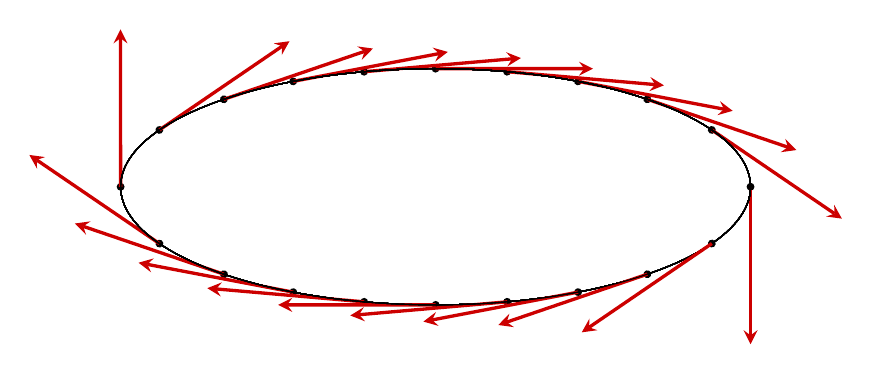
\begin{tikzpicture}
      \coordinate (C) at (3.7,2);
      \foreach \x in {0,0.05,...,0.99}{
        \draw[tangent = \x] (C) ellipse (4 and 1.5);
        \fill[use tangent] (0,0) circle (0.05);
        \draw[red!80!black, ->, use tangent, very thick] (0,0) -- (-2,0);
      }
    \end{tikzpicture}

    Tangent to the curve
  \end{center}
\end{frame}


\begin{frame}{Acceleration for motion with constant speed}
  One way of subtracting vectors, tail-to-tail
  \begin{center}
    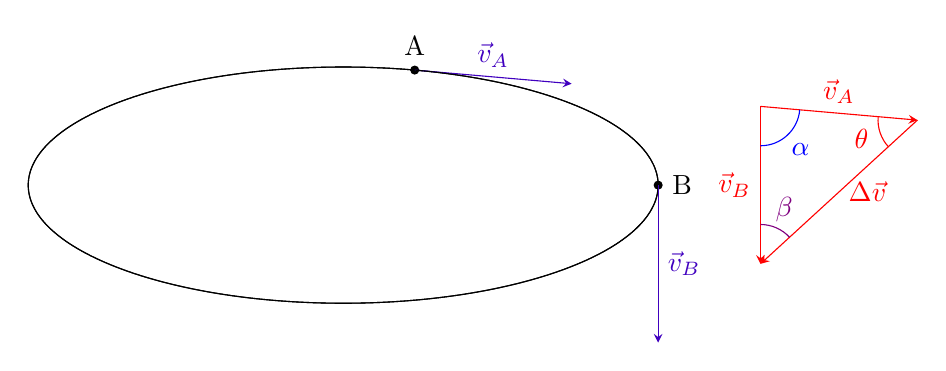
\begin{tikzpicture}
      \def\start{0.2}
      \def\stop{0}
      \def\speed{2}
      
      \coordinate (O) at (0,0);
      \coordinate (C) at (3.7,2);
      \draw[tangent = \start] (C) ellipse (4 and 1.5);
      \node[use tangent,coord] (A) at (0,0) {};
      \node [above] at (A.north) {A};
      \draw[blue!50!violet, ->, use tangent] (0,0) -- (-\speed,0) node[midway,above]{$\vec{v}_A$};
      
      \draw[tangent = \stop] (C) ellipse (4 and 1.5);
      \node[use tangent,coord] (B) at (0,0) {};
      \node [right] at (B.east) {B};
      \draw[blue!50!violet, ->, use tangent] (0,0) -- (-\speed,0)
      node[midway,right]{$\vec{v}_B$};
      
      \coordinate (P) at (9,3);
      \coordinate (va) at ($(P) + (355:2)$);
      \coordinate (vb) at ($(P) + (270:2)$);
      \begin{scope}[red]
        \draw[->] (P) -- +(355:2) node[midway, above]{$\vec{v}_A$};
        \draw[->] (P) -- +(270:2) node[midway, left]{$\vec{v}_B$};
        \draw[->] ($(P) + (355:2)$) -- ($(P) + (270:2)$) node[midway,right]{$\Delta\vec{v}$};
        \draw pic ["$\alpha$", draw, blue, angle eccentricity=1.5] {angle= vb--P--va};
        \draw pic ["$\beta$", draw, violet, angle eccentricity=1.5] {angle= va--vb--P};
        \draw pic ["$\theta$", draw, angle eccentricity=1.5] {angle= P--va--vb};
      \end{scope}
    \end{tikzpicture}
    Questions to consider in \textrm{II}.B
    \begin{itemize}
      \item How are the angles $\alpha, \beta,$ and $\theta$ related?
      \item How are the magnitudes of $\vec{v}_A$ and $\vec{v}_B$ related?
      \item As point B moves closer to point A, what happens to the angles and magnitudes
      mentioned above?
    \end{itemize}
  \end{center}
\end{frame}

\begin{frame}
  {Velocity and Acceleration for constant speed}
  For constant speed:
  
  \begin{center}
    \begin{tikzpicture}
      \coordinate (O) at (0,0);
      \coordinate (V) at (3,0);
      \coordinate (A) at (0,-2);
      \draw[->] (0,0) -- (3,0) node[midway, above]{$\vec{v}$};
      \draw[->] (0,0) -- (0,-2) node[midway, left]{$\vec{a}$};
      \draw (0,-0.3) -- (0.3,-0.3) -- (0.3,0);
    \end{tikzpicture}
  \end{center}
\end{frame}
\end{document}